\chapter{The standard model and beyond}
\label{chap:theory}

\epigraph{It doesn’t stop being magic just because you know how it works.}{--- Terry Pratchett}

\initial{T}his thesis is comprised of experimental searches for dark matter and new physics. The experimental chapter Chpt.~\ref{chap:higgstoinv} delves deeply into the predominantly-featured search for an invisibly decaying Higgs boson. A small chapter is dedicated to the pursuit of \glspl{svj} with Chpt.~\ref{chap:svj}. Before either of which, the theoretical and phenomenological motivations must be understood to corroborate the need for them at the \acrlong{lhc}. In this chapter, a brief recap of the \acrlong{sm}---with emphasis on the Higgs mechanism---will be presented along with its shortcomings, foremost the lack of a dark matter candidate. Theoretical descriptions of dark matter that best fit the relic density and astrophysical observations will then be discussed. Specific interpretations in the forms of \glspl{svj} and invisibly decaying Higgs bosons are examined that provide the background for the respective analysis chapters.


%=========================================================


\section{The standard model of particle physics}
\label{sec:theory_standardmodel}

% Link to objects chapter on electron volts somewhere here (Chpt.~\ref{subsec:objects_electron_volt})

The \acrlong{sm} of particle physics (\acrshort{sm}) is the best description of nature the human race has to offer. Three of the four fundamental forces are encapsulated by it: the strong (nuclear) force, the weak (nuclear) force, and electromagnetism.\footnote{Add a table of the relative strengths and ranges of the forces?} The latter two may instead be considered components of a single \emph{electroweak} force, unified above an energy of $\order{\text{100}\GeV}$; the \acrshort{lhc} above this threshold observes much electroweak physics. All of the elementary particles---the quarks, leptons, gauge bosons, and the Higgs boson---and their interactions with each other are contained within the \acrlong{sm}. These are described initially in Chpt.~\ref{subsec:theory_sm_particles}. Then, in Chpt.~\ref{subsec:theory_higgs_mechanism}, the Higgs mechanism and its eponymous boson, and how they factor in to the decomposition of the electroweak force into the electromagnetic and weak forces are explained.


%=========================================================


\subsection{Particles of the standard model}
\label{subsec:theory_sm_particles}

The \acrlong{sm} contains a relatively small, but diverse ``zoo'' of particles. They can be divided into two distinct categories based on their internal property \emph{spin}: fermions with half-integer spin, comprising the quarks and leptons that constitute matter; and bosons with integer spin, mediating the interactions, i.e., forces, between themselves and fermions.

Six types, or \emph{flavours}, of quarks and six flavours of leptons exist, arranged in three generations. Particles between generations share many similarities, the largest differentiator being mass. In the quark sector, the first generation contains the up \Pup and down \Pdown, the second the charm \Pcharm and strange \Pstrange, and the third the top \Ptop and bottom \Pbottom. The first particle in each generation carries an electric charge of $+\text{2/3}$ of the elementary charge $\Pe$ while the second a value of $-\text{1/3}$. All quarks also carry colour charge, allowing them to combine into colour-neutral composite \emph{hadron} particles such as protons and neutrons.

In the lepton sector, each generation consists of a massive particle with electric charge $-\text{1}\Pe$, and an associated electrically neutral, and extremely light, neutrino. The three generations consist of the electron \Pe and electron neutrino \Pnue, the muon \Pmu and muon neutrino \Pnum, and the tau \Ptau with the tau neutrino \Pnut. The main properties of the fermions are summarised in Tab.~\ref{tab:fermions}.

%Each fermion---with the possible exception of neutrinos---also has a distinct antiparticle, possessing opposite physical charges (such as electrical charge) but otherwise identical properties. The are summarised in Tab.~\ref{tab:fermions}.

\begin{table}[htbp]
    \centering
    \begin{tabular}{cclccr}
        \hline\hline
        Type & Generation & Particle & Spin & Electric charge & Mass \\ \hline
        \multirow{6}{*}{Quark} & \multirow{2}{*}{1} & Up (\Pup) & 1/2 & $+$2/3\,\Pe & 2.2$^{+\text{0.5}}_{-\text{0.4}} \MeVcc$ \\
        & & Down (\Pdown) & 1/2 & $-$1/3\,\Pe & 4.7$^{+\text{0.5}}_{-\text{0.3}} \MeVcc$ \\
        & \multirow{2}{*}{2} & Charm (\Pcharm) & 1/2 & $+$2/3\,\Pe & 1.28$^{+\text{0.03}}_{-\text{0.04}} \GeVcc$ \\
        & & Strange (\Pstrange) & 1/2 & $-$1/3\,\Pe & 95$^{+\text{9}}_{-\text{3}} \MeVcc$ \\
        & \multirow{2}{*}{3} & Top (\Ptop) & 1/2 & $+$2/3\,\Pe & 173$\pm \text{0.4} \GeVcc$\\
        & & Bottom (\Pbottom) & 1/2 & $-$1/3\,\Pe & 4.18$^{+\text{0.04}}_{-\text{0.03}} \GeVcc$ \\ \hline
        \multirow{6}{*}{Lepton} & \multirow{2}{*}{1} & Electron (\Pe) & 1/2 & $-$1\,\Pe & 0.511\MeVcc \\
        & & Electron neutrino (\Pnue) & 1/2 & 0 & $< \text{0.2\eVcc}$ \\
        & \multirow{2}{*}{2} & Muon (\Pmu) & 1/2 & $-$1\,\Pe & 106\MeVcc \\
        & & Muon neutrino (\Pnum) & 1/2 & 0 & $< \text{0.2\eVcc}$ \\
        & \multirow{2}{*}{3} & Tau (\Ptau) & 1/2 & $-$1\,\Pe & 1.777\GeVcc \\
        & & Tau neutrino (\Pnut) & 1/2 & 0 & $< \text{0.2\eVcc}$ \\ \hline\hline
    \end{tabular}
    \caption[A summary of the fermionic particles of the standard model]{A summary of the fermionic particles of the \acrlong{sm}. Masses obtained from Ref.~\citenum{PhysRevD.98.030001}.}
    \label{tab:fermions}
\end{table}

Each force contains one or more spin-1 gauge bosons mediating the fermions' interactions. Eight flavours of the massless, electrically neutral gluon \Pgluon carries the strong force, while the equally massless and chargeless photon \Pphoton mediates the electromagnetic interaction. Three massive bosons mediate the weak interaction, the charged \PWpm and neutral \PZ. A scalar (spin-0) Higgs boson \PH mediates the Higgs field that acts to bestow mass to the elementary particles. All of the bosons are summarised in Tab.~\ref{tab:bosons}.

\begin{table}[htbp]
    \centering
    \begin{tabular}{clccr}
        \hline
        Force & Particle & Spin & Electric charge & Mass \\ \hline
        Strong & Gluon (\Pgluon) & 1 & 0 & 0 \\
        Electromagnetism & Photon (\Pphoton) & 1 & 0 & 0 \\
        Weak & \PW bosons (\PWpm) & 1 & $\pm$1\,\Pe & $\text{80.38} \pm \text{0.01}\GeVcc$ \\
        Weak & \PZ boson (\PZ) & 1 & 0 & 91.19\GeVcc \\
        --- & Higgs boson (\PH) & 0 & 0 & $\text{125.18} \pm \text{0.16}\GeVcc$ \\ \hline
    \end{tabular}
    \caption[A summary of the bosonic particles of the standard model]{A summary of the bosonic particles of the \acrlong{sm}. Masses obtained from Ref.~\citenum{PhysRevD.98.030001}.}
    \label{tab:bosons}
\end{table}


%=========================================================


\subsection{Symmetries and gauge invariance}

The \acrlong{sm} is a gauge quantum field theory: particles are characterised by quantum fields and their interactions described by continuous gauge symmetry groups. A symmetry is a feature in a theory where a quantity is preserved under specific transformations. This is significant for understanding what interactions are allowed by each force. An SU(3) gauge group represents the interactions in the strong force, and a $\text{SU(2)} \times \text{U(1)}$ gauge group for the electroweak force. Decomposition into the weak force and electromagnetism results in separate SU(2) and U(1) groups, respectively. The interactions of the \acrlong{sm} as a whole can then be expressed as the product $\text{SU(3)} \times \text{SU(2)} \times \text{U(1)}$.

Noether's theorem associates a continuous symmetry of a physical system, that does not affect its Lagrangian, to a conserved charge or current~\cite{Noether_1971}. A consequence of which that an interaction represented by a particular group must conserve the charges associated to the symmetries of said group. The generators of the group\footnote{There are $N^2 - \text{1}$ generators for SU($N$) and $N^2$ for U($N$). This is what gives rise to the eight gluons of the strong force, three \PWplus, \PWminus, and \PZ bosons of the weak force, and the single photon of electromagnetism.} correspond to the gauge invariant fields that mediate the associated force, i.e., the gauge bosons in the \acrshort{sm}, enforcing the conservation of the charges.\footnote{Not entirely sure if this bit is correct, since e.g., electromagnetism must conserve charge but the photon doesn't carry charge.} With the SU(3) strong force, the mediating gluons carry colour charge. The photon \Pphoton mediating U(1) electromagnetism conserves electrical charge. While the bosons of the SU(2) weak force that conserve weak isospin. As the \acrshort{sm} is described by the product of these gauge groups, it includes only gauge invariant fields that preserve the Lagrangian and equations of motions under the allowed transformations or interactions.

Symmetries in the \acrlong{sm} require the gauge bosons. For electromagnetism and the strong force, this is no issue. However, the bosons mediating the weak force have been determined experimentally to be massive~\cite{Arnison:1983mk,Bagnaia:1983zx}, posing a problem. One solution is to introduce a new field that can break the symmetry of the SU(2) group without affecting the gauge invariance elsewhere in the \acrshort{sm}. This led to the creation of the Higgs field.\footnote{There are many who deserve credit for formulating the theory. However, for concision, it will be referred to as the \emph{Higgs field} or \emph{Higgs mechanism} henceforth.}

% In the lepton sector, each generation consists of a doublet of left-handed chiral states $(\Pnu_{\mathrm{L}}, \Plepton_{\mathrm{L}})$ arising from the SU(2) weak isospin symmetry, and a singlet of right-handed chiral states $\Plepton_{\mathrm{R}}$.


%=========================================================


\subsection{Electroweak symmetry breaking and the Higgs mechanism}
\label{subsec:theory_higgs_mechanism}

% Basically talk through the foundation of the Higgs mechanism a bit, citing the 1964 papers. Show mathematically what the Higgs scalar field is, and what the potential is (with a plot). Then talk about what the symmetry breaking does and how the weak bosons get their mass. I guess also talk about how the fermions get their masses (since, while it's the Higgs field that gives it, it's not strictly the Higgs 'mechanism' as that term is reserved for how the weak bosons get their masses). Then make sure this section flows into the SM limitations bit and also doesn't overlap with the Hinv section

As mentioned earlier, the electromagnetic and weak forces are unified into one above an energy threshold. In this regime, the electroweak bosons and fermions must be massless to maintain gauge invariance. The electroweak bosons obtain their mass by interacting with the Higgs field, the mechanism through which is labelled the \emph{Higgs mechanism}~\cite{PhysRevLett.13.321,PhysRevLett.13.508,PhysRevLett.13.585}.\footnote{The fermions (except perhaps neutrinos), also obtain their masses from interacting with the Higgs field. However, the term ``Higgs mechanism'' in the \acrlong{sm} is reserved for the procedure by which the electroweak bosons acquire mass.} 

The simplest model by which the Higgs mechanism can be accommodated in the \acrshort{sm} is by introducing an SU(2) doublet of complex scalar Higgs fields:
\begin{equation}
    \HiggsField = \begin{pmatrix} \phi^+ \\ \phi^0 \end{pmatrix} = \frac{1}{\sqrt{2}} \begin{pmatrix} \phi_1 + i\phi_2 \\ \phi_3 + i\phi_4 \end{pmatrix}
    \label{eq:higgs_field}
\end{equation}

It possesses four degrees of freedom, i.e., one per gauge boson in the electroweak sector. The fields introduce additional terms in the \acrlong{sm} Lagrangian, most importantly a potential of the form
\begin{equation}
    V(\HiggsField) = \mu^2 \HiggsField^{\dagger} \HiggsField - \lambda (\HiggsField^{\dagger} \HiggsField)^2
    \label{eq:higgs_potential}
\end{equation}

which is the most general scalar potential that is also $\text{SU(2)} \times \text{U(1)}$ invariant. By setting $\lambda < 0$ and $\mu^2 < 0$, a degenerate circle of minima in the $\phi_1\text{--}\phi_2$ plane can be found with values
\begin{equation}
    \HiggsField^{\dagger} \HiggsField \lvert_{\mathrm{min}} = \frac{\mu^2}{2\lambda}
    \label{eq:higgs_mu_lambda}
\end{equation}

and the familiar ``wine bottle'' potential is formed. An illustration of the potential with a Higgs boson is given in Fig.~\ref{fig:higgs_potential}.

\begin{figure}[htbp]
    \centering
    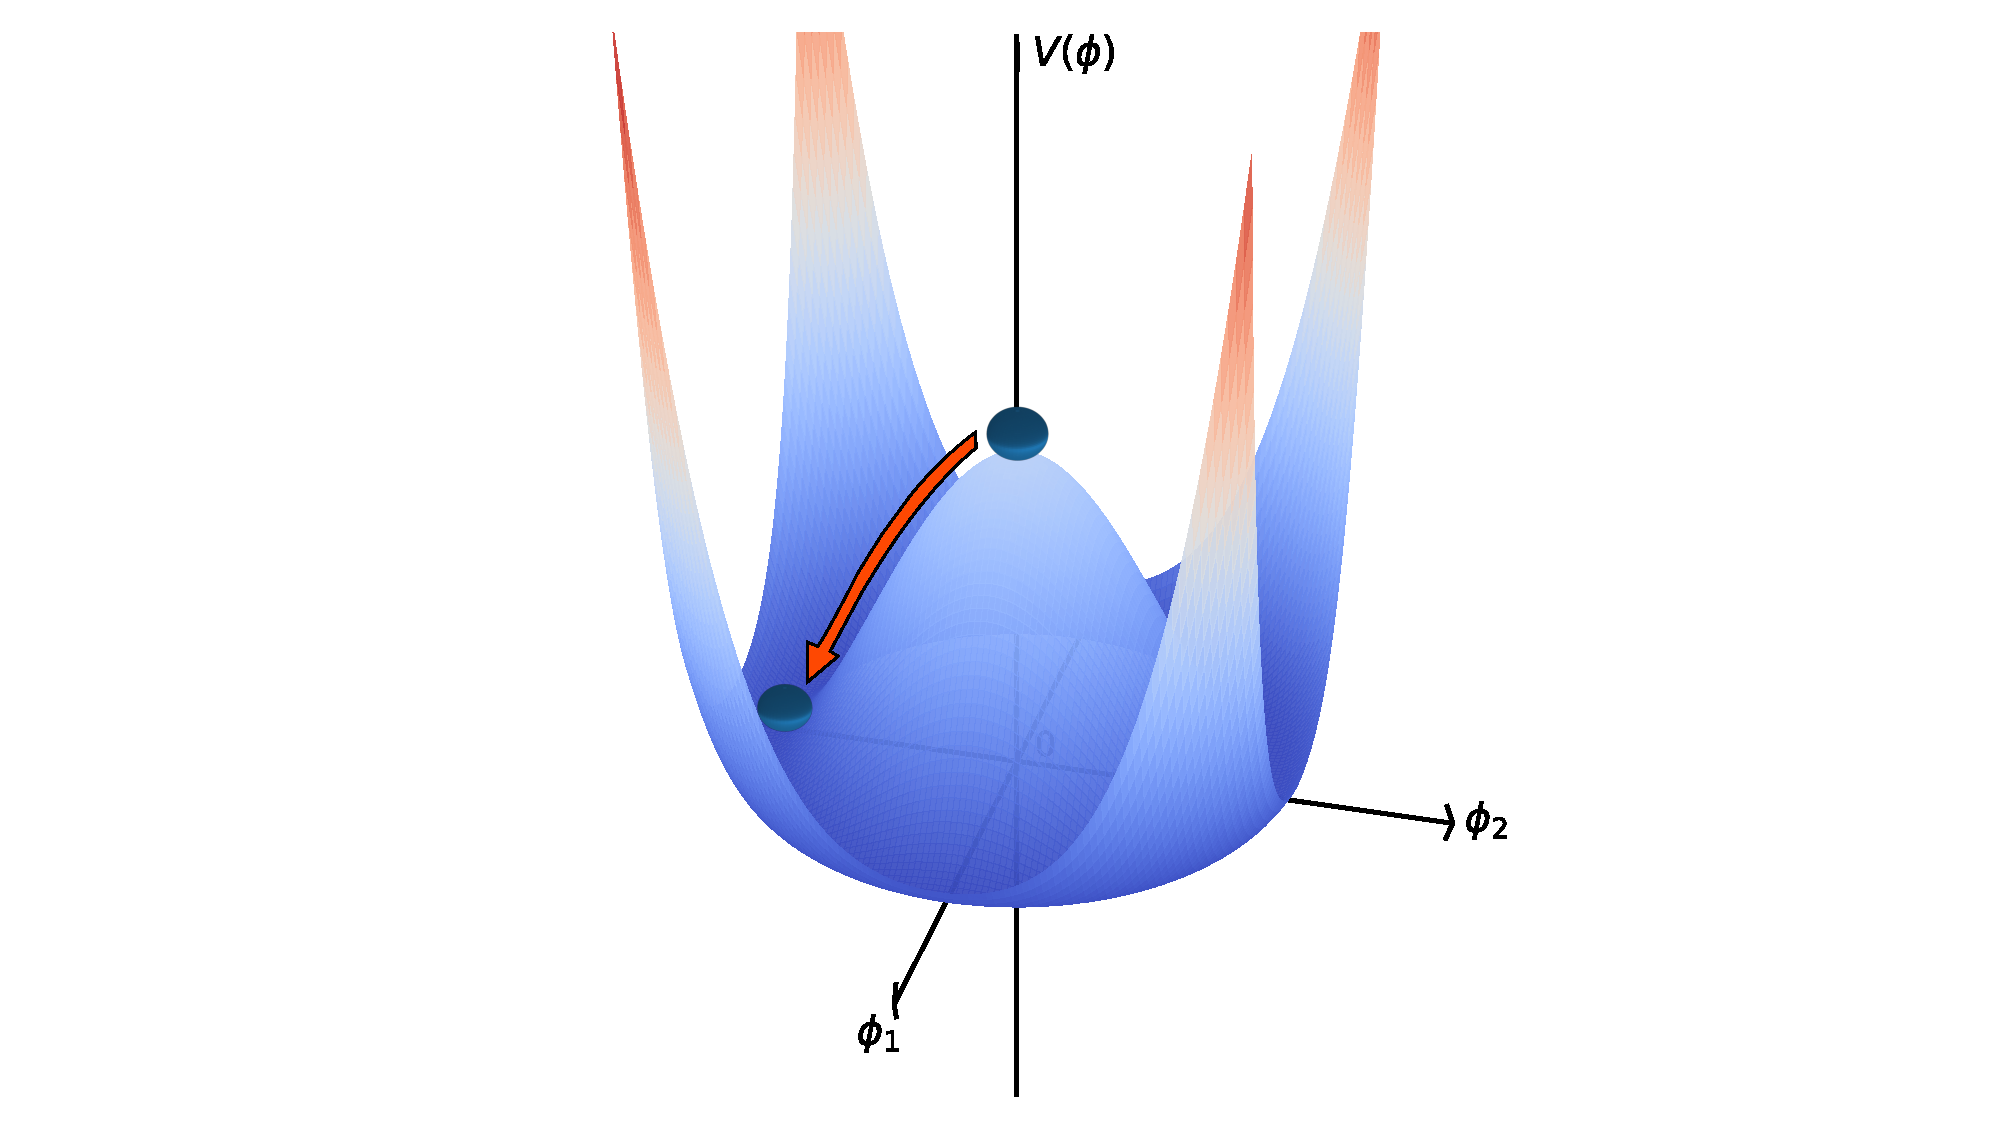
\includegraphics[width=0.5\textwidth]{./figures/higgs_potential_from_pptx.pdf}
    \caption[A depiction of the Higgs potential $V$ as a function of the component fields. The Higgs boson is initially at $(\phi_1, \phi_2) = (0, 0)$, then tumbles into the minimum value of $V$ at the point of electroweak symmetry breaking]{A depiction of the Higgs potential $V$ as a function of the component fields. The Higgs boson is initially at $(\phi_1, \phi_2) = (0, 0)$, then tumbles into the minimum value of $V$ at the point of electroweak symmetry breaking.}
    \label{fig:higgs_potential}
\end{figure}

They, along with the photon, are instead represented as $\PW_1$, $\PW_2$, and $\PW_3$ boson fields carrying weak isospin, and the $B$ boson field of weak hypercharge.\footnote{Actually explain how electroweak symmetry breaking happens here. Make sure to reference the 1964 papers.} At energies below electroweak unification, the Higgs mechanism spontaneously breaks the $\text{SU(2)} \times \text{U(1)}$ symmetry, decoupling electromagnetism from the weak force. The $\PW_1$ and $\PW_2$ fields transform into \PWplus and \PWminus bosons, gaining their 80\GeV mass:
\begin{equation}
    \PWpm = \frac{1}{\sqrt{2}} (\PW_1 \mp i\PW_2)
    \label{eq:EWSB_W}
\end{equation}

While the $\PW_3$ and $B$ fields mix to produce the massless photon and massive \PZ boson:
\begin{equation}
    \begin{pmatrix} \Pphoton \\ \PZ \end{pmatrix} = \begin{pmatrix} \cos\thetaW & \sin\thetaW \\ -\sin\thetaW & \cos\thetaW \end{pmatrix} \begin{pmatrix} B \\ \PW_3 \end{pmatrix}
    \label{eq:EWSB_photon_Z}
\end{equation}

where \thetaW is the weak mixing angle, defined as
\begin{equation}
    \cos\thetaW = \frac{m_{\PW}}{m_{\PZ}}
    \label{eq:weak_mixing_angle}
\end{equation}

Its value is constrained by experiment. In the new U(1) symmetry group of electromagnetism, the electric charge quantum number manifests as a combination of weak hypercharge and a component of weak isospin.

\begin{easylist}[itemize]
    \easylistprops
    & If I need to make a Higgs potential plot or something, can try with \url{https://www.transum.org/Maths/Activity/Graph/Desmos.asp} if I want something interactive. Otherwise, can probs make a 3D plot with matplotlib
    && Mention resonances and widths. Each decay mode of a particle contributes a partial width (which determines its branching ratio: \BR = partial width/total width).
    && Talk in some detail about the Higgs mechanism as that will inform the Higgs to invisible section. Mention Yukawa coupling to fermions, and that it's dependent on the squared mass of the decay products. Lends credence to suppression of direct decay to neutrinos (assuming they even couple to Higgs).
\end{easylist}

% Check Lancaster and other summer school notes (Postgraduate and CMS courses/ folder)
% What I could do is present a recap/highlight the main points of the standard model (collection of QFT-derived components, note the group theory stuff).


%=========================================================


\subsection{Limitations of the standard model}
\label{subsec:sm_limitations}

% Check Lancaster and other summer school notes for other limitations, specifically referencing things that can tie into dark matter

Despite the \acrlong{sm} providing precise predictions of three of the four fundamental forces and the particles that they interact with, there are many experimental observations that it cannot currently explain. Neutrino masses, dark matter, dark energy, and gravity all escape its description.

The Hierarchy Problem is one of the more serious issues facing the \acrlong{sm}. It may be explained in different manners that emphasize certain aspects. But inherently, it is a question of the disparity between energy scales of the fundamental forces---particularly relating to the weak force and gravity. The masses of the intermediate vector, and Higgs, bosons of $\order{\text{100}\GeVcc}$ are much smaller than than the Planck mass of $\order{\text{10}^{19}\GeVcc}$. The mass term for the Higgs boson is $m^2 \phi^{\dagger} \phi$ in the \acrshort{sm}. Invariance under a gauge or global symmetry in the Higgs field $H$ leads to the mass being open to radiative corrections up to the Plank scale.\footnote{Justify this more?} It appears that, in nature, these very large corrective terms to the Higgs boson mass cancel to give the familiar $m_{\PH} = \text{125}\GeVcc$~\cite{Chatrchyan:2012xdj,Aad:2012tfa}. It is deemed unnatural to expect cancellations to such a degree, i.e., one part in 10$^{17}$. This \emph{fine-tuning} of parameters in the \acrlong{sm} is something that unified or natural theories desperately try to avoid.

Some \acrshort{bsm} theories like \acrlong{susy} provide well-motivated cancellations by introducing supersymmetric particles. In certain scenarios, some of these particles should exist at the \TeVns scale. In the \acrshort{sm}, the largest correction to the Higgs mass derives from the top quark, since its Yukawa coupling to the Higgs is the strongest. At one-loop order, new physics at $\order{\TeVns}$ scale is required, with new particles coupling to the Higgs field to prevent these corrections from being unreasonably large~\cite{Farina:2013ssa}. Arguments such as this give credence to new physics being discoverable at particle accelerators such as the \acrlong{lhc}.


%=========================================================


\section{Theoretical motivations for, and descriptions of, dark matter}
\label{sec:theory_dark_matter}

% See dark matter lecture notes from STFC summer school for expanded info.

Dark matter may have been forged in the universe via one of many possible mechanisms. The most popular is described as a \emph{thermal freeze-out} process. In the hot, early universe when the thermal background allowed spontaneous pair production of particle dark matter, it was generated in abundance. During this period, the particles may also have frequently annihilated seeing that the cosmos was still small. Inevitably, the universe expanded and cooled; the temperature became too low to allow significant production~\cite{Baldes:2017gzw}. Matter was further separated and the dark matter annihilation rate decreased, leaving a behind the \emph{thermal relic} that is observed today. These remaining particles were attracted via gravity, forming filaments throughout the universe. The potential wells they induced allowed the progenitors of galaxies to form within.

Full derivations of the thermal freeze-out of dark matter can be found in literature~\cite{cosmic_abundances_stable_particles,Bender:2012gc}, with the \acrshort{wimp} Miracle as a consequence: with relatively few assumptions, the correct dark matter relic abundance can be recovered by requiring a \acrshort{wimp} mass of $\order{\text{\GeVns--\TeVns}}$, dependent on the annihilation cross section. This is a range accessible at contemporary colliders such as the \acrshort{lhc}, and perhaps coincidentally, around the electroweak energy scale. It is common for figures that depict the \acrshort{wimp} dark matter density over time to plot the yield $n_{\chi}/s$ as a function of the dimensionless parameter $x = m_{\chi}/T$. In the former variable, $n_{\chi}$ is the number density and $s$ is the entropy density. In the latter, $m_{\chi}$ is the dark matter mass and $T$ is the average temperature of the universe, which serves as a measure of its age due to the temperature decreasing over time. An example is given in Fig.~\ref{fig:theory_dm_abundance}.

\begin{figure}[htbp]
    \centering
    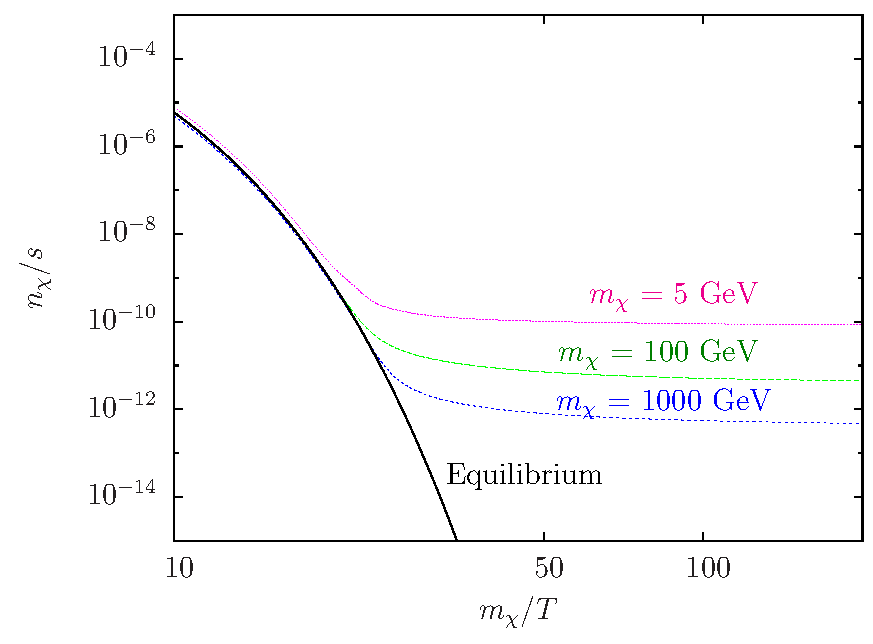
\includegraphics[width=0.75\textwidth]{figures/dm_abundance.pdf}
    \caption[A measure of the comoving number density of \acrshort{wimp} dark matter as a function of time with projections for different particle masses]{A measure of the comoving number density of \acrshort{wimp} dark matter as a function of time with projections for different particle masses. A higher mass must be balanced by a larger annihilation cross section to achieve the correct relic density, to which it tends asymptotically from the point of decoupling. The black curve represents the scenario in which dark matter remains in equilibrium with the \acrlong{sm}. Figure taken from Ref.~\citenum{Han:2013gba}.}
    \label{fig:theory_dm_abundance}
\end{figure}

The time of the dark matter freeze out epoch is somewhat insensitive to the mass and annihilation cross section. Approximate solutions to the Boltzmann equation for time-dependent $n_{\chi}$---where dark matter is modelled as a weakly-interacting, diffuse gas of particles---suggest $x_f \sim 20$~\cite{Lisanti:2016jxe,Bender:2012gc}. Stronger dark matter interaction leads to decoupling at a later time and a lower number density. The approximate value of $x_f$ is significant in that it supports the electroweak-scale mass of \glspl{wimp}.

Another popular mechanism, targeting low-mass dark matter, is the \emph{freeze-in} process~\cite{Hall:2009bx,Krnjaic:2017tio}. In this postulate, dark matter is not produced thermally in the early universe. Instead, it emerges through interactions between \acrshort{sm} particles such as collisions, or decays of those heavier than dark matter. The comoving density increases with time until it plateaus from of the cooling of the universe, where \acrshort{sm} particles are generally stable enough and too low energy to produce dark matter in any meaningful quantity. The relic abundance can therefore reclaimed from a combination of the initial thermal distributions, the dark matter mass, and the interaction strength, similar to the freeze-out process. In order to obey cosmological observations, particularly the fact that it is cold, the masses expected for freeze-in dark matter particles are of $\order{\keVns}$ or heavier.


%=========================================================


\section{Measuring the branching ratio of invisibly decaying Higgs bosons}
\label{sec:theory_higgs_to_inv}

The Higgs boson has caught the attention of the high energy physics community, and even the public eye, like no other particle in recent memory. Its discovery in the $\HepProcess{\PH \to \Pphoton\Pphoton}$ and $\HepProcess{\PH \to \PZ\PZ \to \text{4}\Plepton}$ channels in 2012---independently by both \acrshort{cms}~\cite{Chatrchyan:2012xdj} and \acrshort{atlas}~\cite{Aad:2012tfa}---realised one of the paramount goals of the \acrshort{lhc}'s construction. The particle itself is not necessarily exciting. Rather, it confirms the existence of the Higgs \emph{field} that pervades the universe and gives mass to the elementary particles via the exchange of its eponymous boson~\cite{PhysRevLett.13.321,PhysRevLett.13.508,PhysRevLett.13.585}. Its discovery, one might think, was the end of the discussion of the Higgs boson. However, it was only the beginning.

Many observations of the Higgs, such as its predominant decay mode $\HepProcess{\PH \to \Pqb\APqb}$, were not seen until recently by \acrshort{cms}~\cite{Sirunyan:2018kst} or \acrshort{atlas}~\cite{Aaboud:2018zhk}. Constraints on its other properties have also been placed, such as its resonance width and branching ratios \BR to several final states. Fully understanding the Higgs boson is important to understanding the Higgs field and the wider \acrlong{sm}. Precision measurements in tension with \acrshort{sm} predictions can also be a window to new physics. Measuring the \higgstoinv branching ratio aims to do just that.

The only \acrshort{sm} process in which Higgs boson can decay invisibly is $\HepProcess{\PH \to \PZ\PZ \to 4\nu}$\footnote{A direct decay to neutrinos is possible if they acquire their mass from the Higgs field. But as the coupling is of a Yukawa form and the upper limit on the \acrshort{sm} neutrino masses is very small, the branching ratio is expected to be heavily suppressed.} with a branching ratio of $\order{\text{0.1\,\%}}$~\cite{Heinemeyer:1559921}. The leading observed experimental upper limits on this measurement are 19\,\% from CMS~\cite{Sirunyan:2018owy} and 26\,\% from \acrshort{atlas}~\cite{Aaboud:2019rtt}, far higher than the predicted value. If undiscovered invisible particles, perhaps dark matter, couple to the Higgs field the branching ratio will be enhanced.\footnote{Do I need to give a more mathematical motivation for the BR being enhanced/what kind of values the BR is expected to be from various DM models?} Experimental evidence shows the coupling strength to proportionally follow the mass of the particle, as verified in \acrshort{atlas} and \acrshort{cms}' latest measurements~\cite{Sopczak:2708121}. A considerably large enhancement may allow for this process to be observed at the \acrshort{lhc}. At the very least, a more accurate constraint on the branching ratio is able to exclude some models of dark matter, such as those described in Refs.~\citenum{Djouadi:2012zc,KAKIZAKI201544}.

There is no reason to assume dark matter does \emph{not} interact with the Higgs field, since it bestows mass to all known elementary particles (a small caveat, perhaps, being neutrinos).\footnote{Do I need to give some mathematical motivation as to \emph{why} dark matter would couple to the Higgs? Or is the fact that it has mass enough justification?} Higgs \emph{portal} models have been theorised that connect the visible sector of the \acrlong{sm} to a dark sector where particle dark matter resides~\cite{higgs_portal_singlet_dm,Arcadi:2019lka}. Certain models also predict a detectable presence at the \acrshort{lhc} from a sufficient production rate~\cite{Boveia:2018yeb}, perhaps even with data obtained during Run-2~\cite{Abercrombie:2015wmb}.

% If models exist, mention briefly about potential theories with dark matter candidates being able to fix the hierarchy problem (present in a mathematical context if possible).

An analysis in search of this decay is provided thoroughly in Chpt.~\ref{chap:higgstoinv}. Constraints on the experimental side stem largely from the different channels in which a Higgs boson can be produced. These are outlined in Chpt.~\ref{subsec:theory_higgs_production_modes}, and must all be considered when examining such a rare process that is also difficult to distinguish amongst a large background. Previous results from searches for individual modes, including subsequent combinations, are documented in Chpt.~\ref{subsec:theory_hinv_prev_results}.


%=========================================================


\subsection{Production modes of the Higgs boson}
\label{subsec:theory_higgs_production_modes}

At the \acrshort{lhc}, the most common mechanisms for producing a Higgs boson are \acrfull{vbf}, gluon-gluon fusion (\ggF or \ggH), associated production from top quarks (\ttH), and associated production from a vector boson (\VH). Feynman diagrams of these processes are shown in Fig.~\ref{fig:higgs_feynman_diagrams}. Additional diagrams for \ggH involve a square top quark loop. The \ZH process can be initiated by $\HepProcess{\Pgluon\Pgluon\to \ZH}$ as well as $\HepProcess{\Pp\Pp \to \ZH}$. They have very different characteristics, production rates, and event signatures, complementing each other and allowing a single analysis to cover all bases with orthogonal parameter spaces to target them individually. One common feature of these final states is the presence of at least one quark. The hadronic constituents in the decay products of a collision often shower due to colour confinement, producing collimated sprays of hadrons called \emph{\glspl{jet}}. In a detector, these are represented by clusters of hadronic energy deposits. Algorithms at each stage of data acquisition (see Chpt.~\ref{subsec:cms_recording_data}) can reliably connect these back to the individual quark decays so one has some certainty of the process they are observing.

\begin{figure}[htbp]
    \centering
    \begin{subfigure}[b]{0.45\textwidth}
        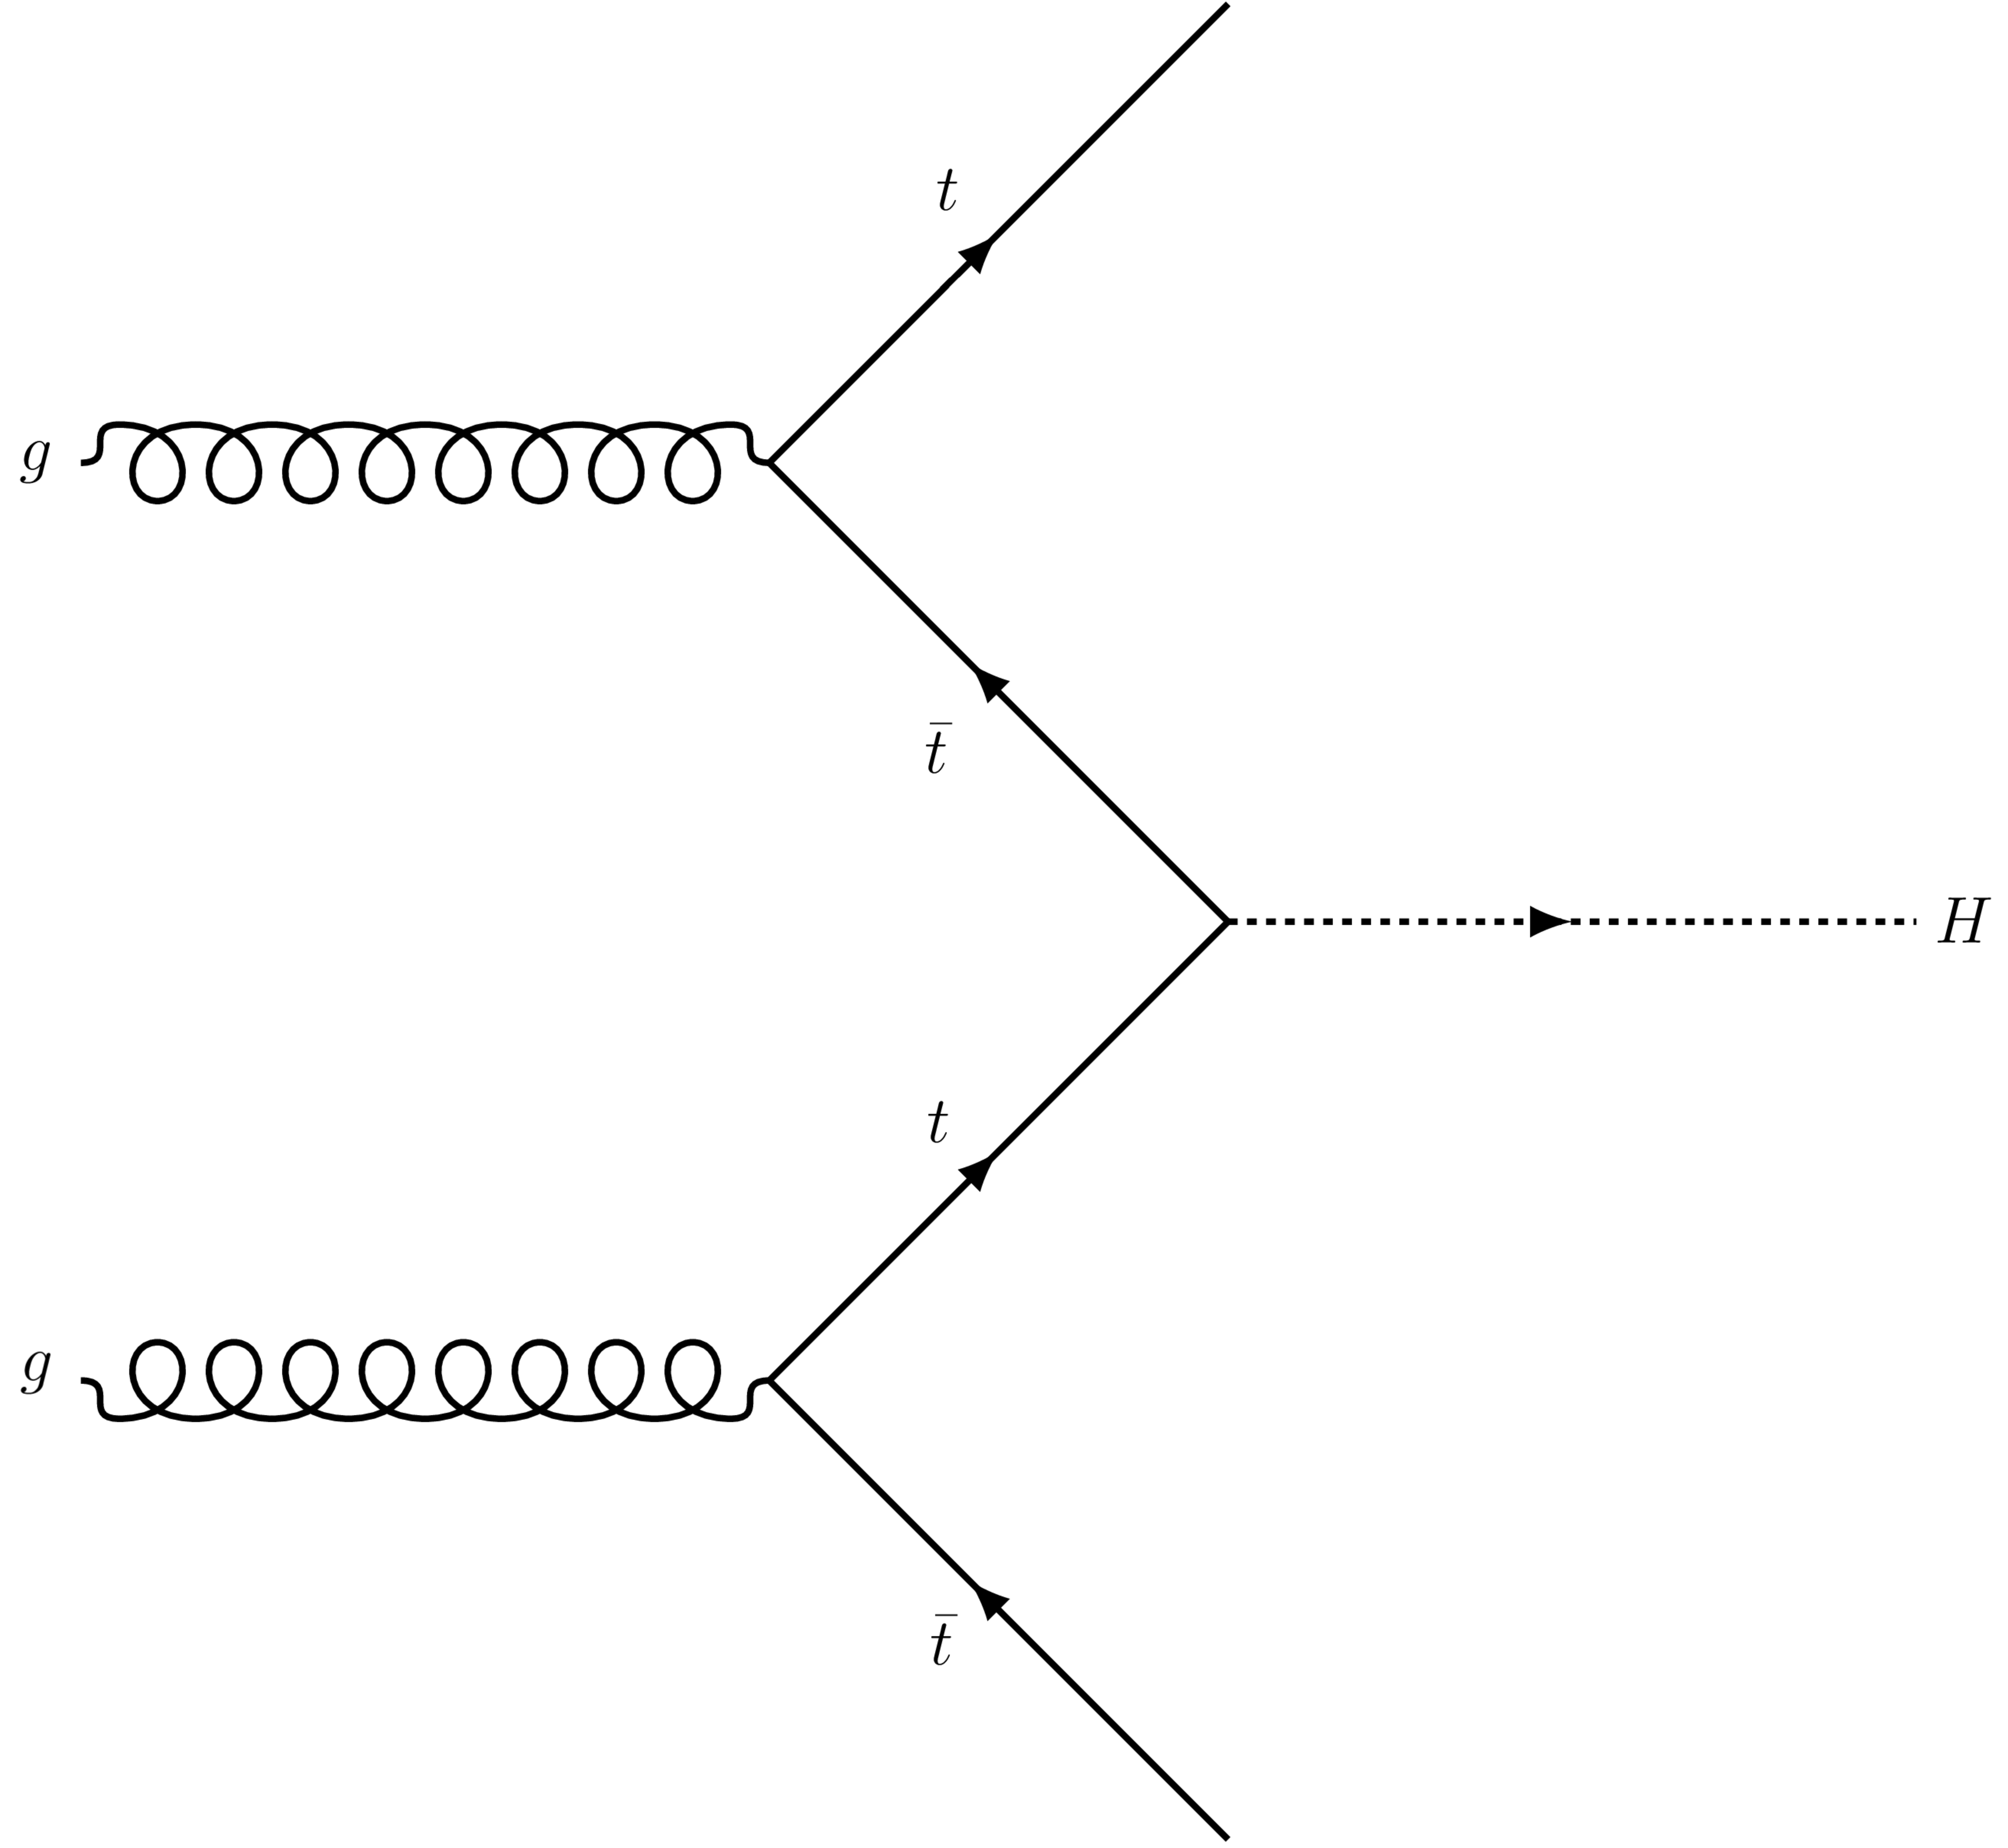
\includegraphics[width=\textwidth]{figures/feynman_diagrams/ttH.pdf}
        \caption{\ttH}
    \end{subfigure}
    \hfill
    \begin{subfigure}[b]{0.45\textwidth}
        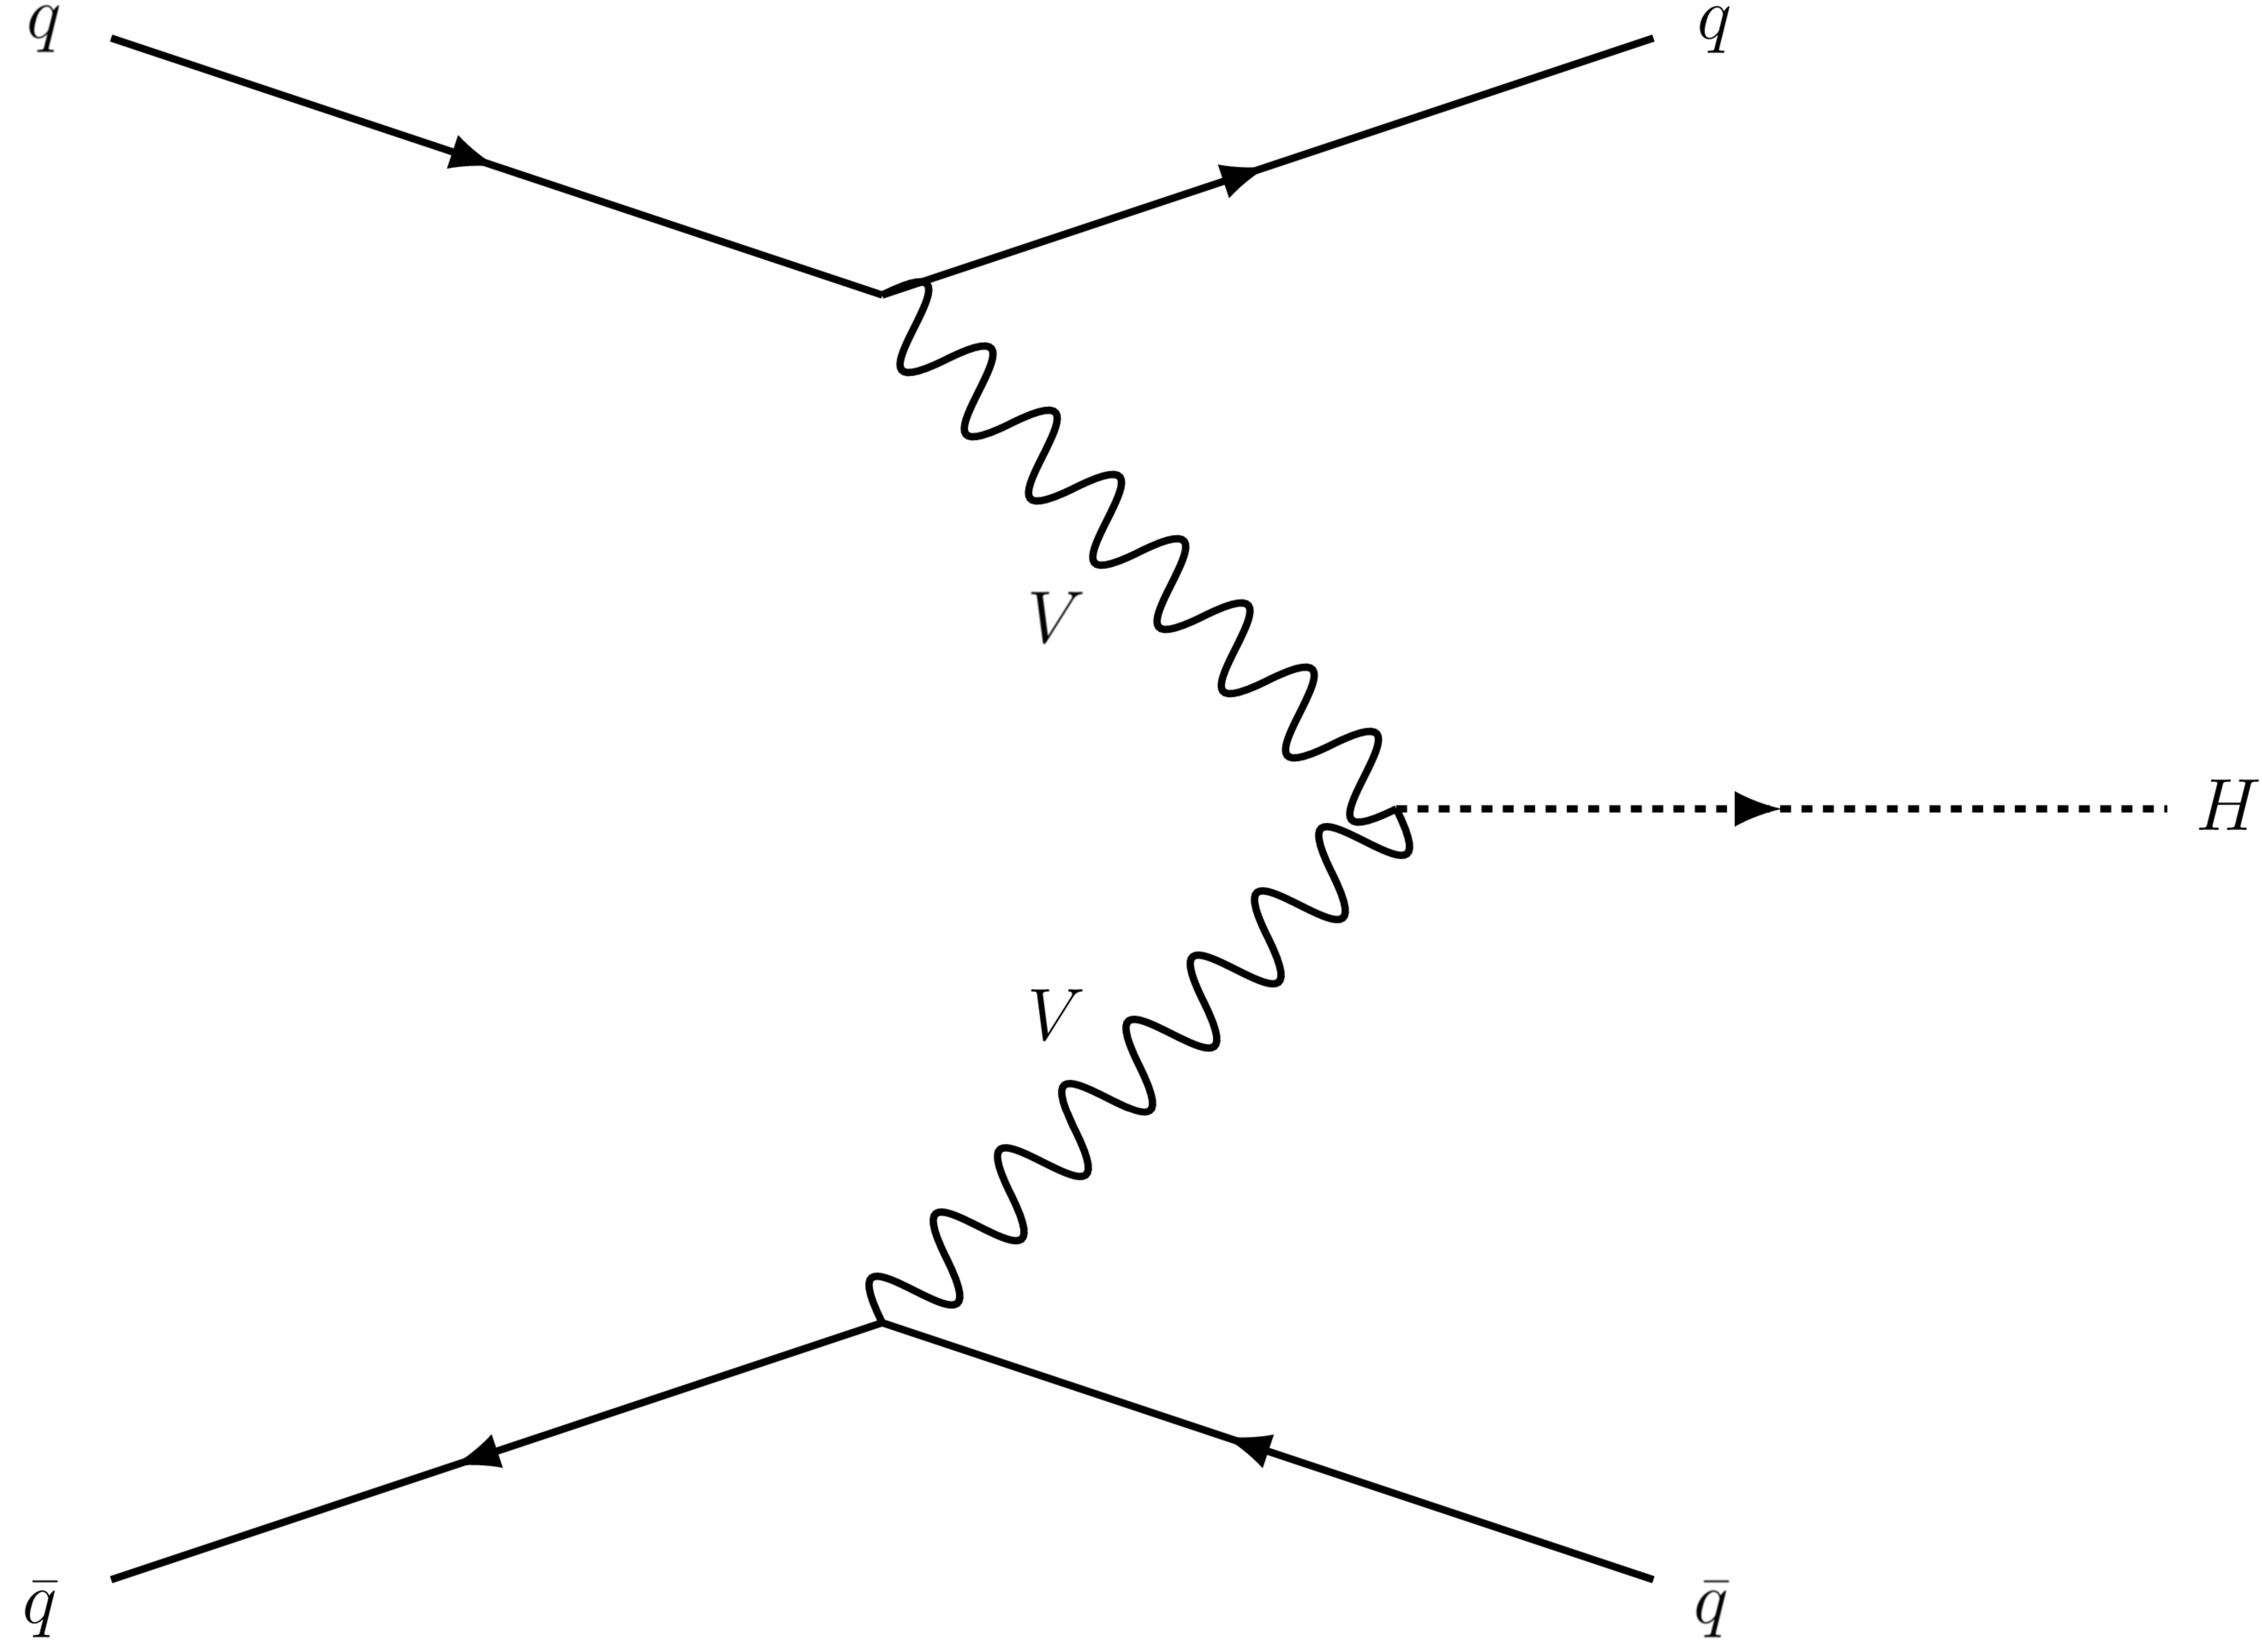
\includegraphics[width=\textwidth]{figures/feynman_diagrams/VBF.pdf}
        \caption{\acrshort{vbf}}
    \end{subfigure}
% blank line to start new row
    \begin{subfigure}[b]{0.45\textwidth}
        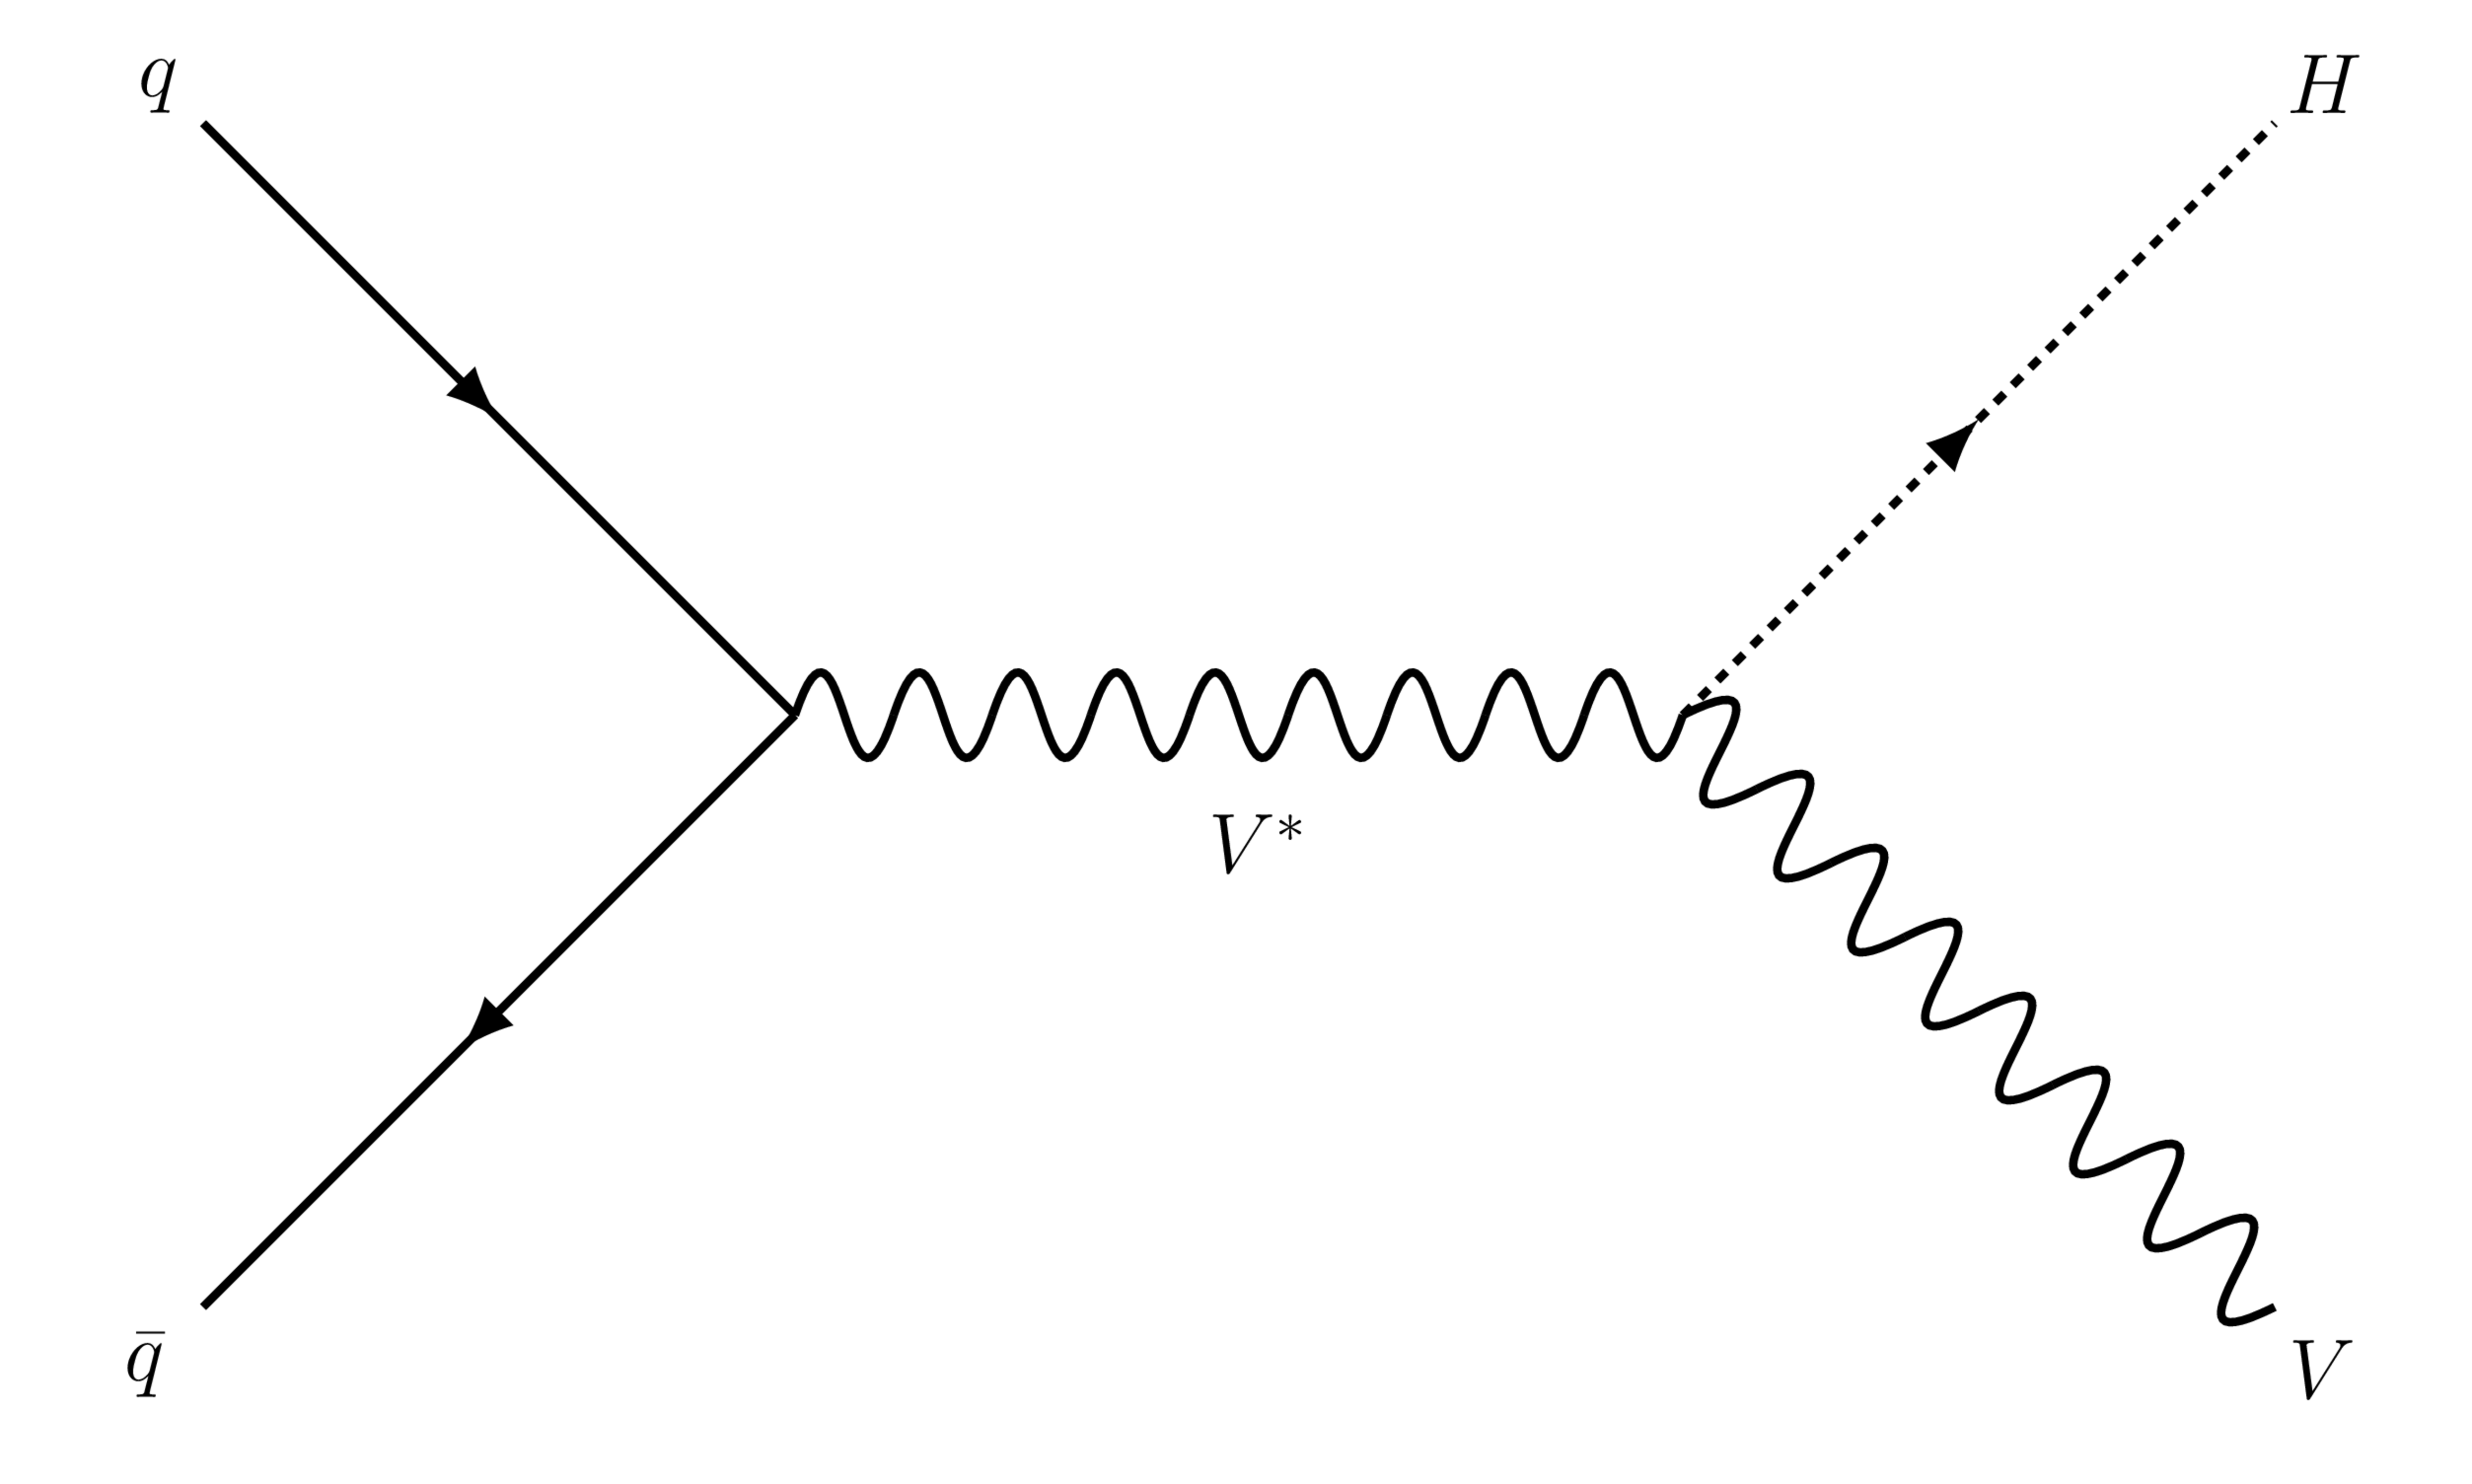
\includegraphics[width=\textwidth]{figures/feynman_diagrams/VH.pdf}
        \caption{\VH}
    \end{subfigure}
    \hfill
    \begin{subfigure}[b]{0.45\textwidth}
        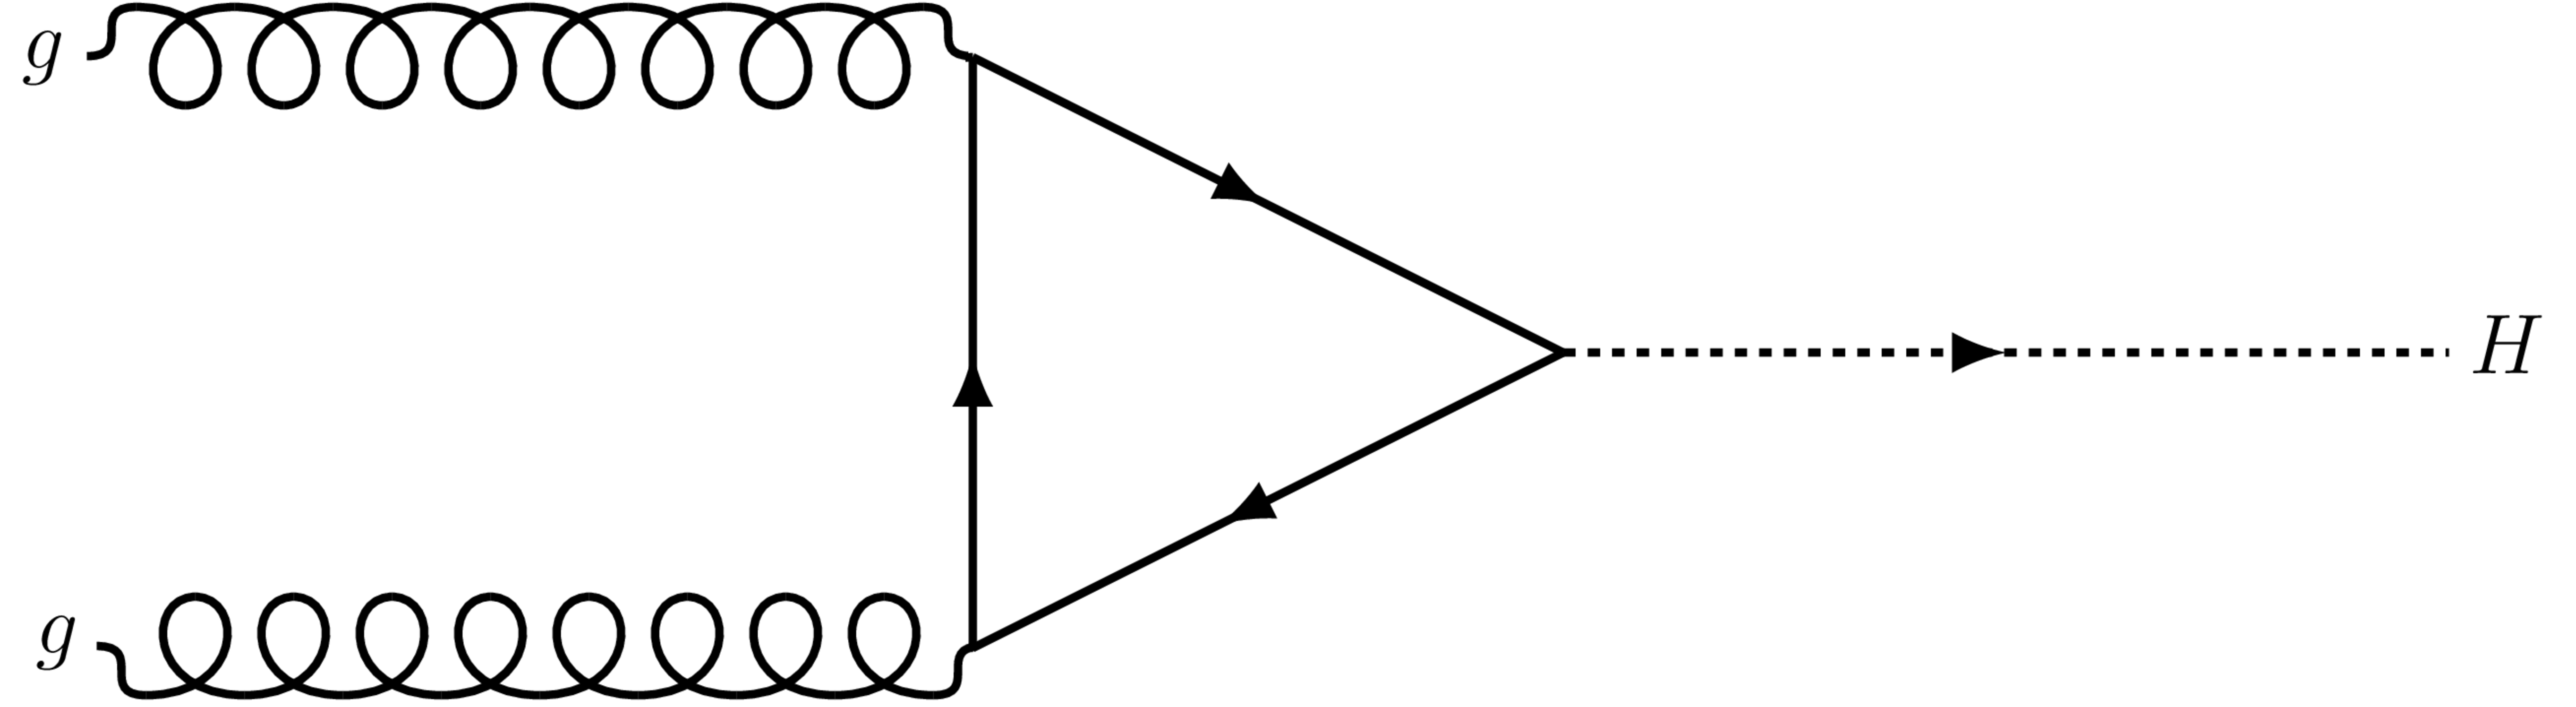
\includegraphics[width=\textwidth]{figures/feynman_diagrams/ggF.pdf}
        \caption{\ggH}
    \end{subfigure}
\caption[A subset of the Feynman diagrams for the four predominant production mechanisms of the Higgs boson at the LHC]{A subset of the Feynman diagrams for the four predominant production mechanisms of the Higgs boson at the \acrshort{lhc}.}
\label{fig:higgs_feynman_diagrams}
\end{figure}

The cross section of each mechanism at \comruntwo is detailed in Tab.~\ref{tab:htoinv_signal_xsecs}.

\begin{table}[htbp]
    \centering
    \begin{tabular}{cll}
        \hline
        Mode (\higgstoinv) & Cross section (pb) & Accuracy \\\hline
        \acrshort{vbf} & 3.77 & \acrshort{nnlo} \acrshort{qcd} and \acrshort{nlo} electroweak \\
        $\ttH$ & $\text{5.07} \times \text{10}^{-1}$ & \acrshort{nlo} \acrshort{qcd} and \acrshort{nlo} electroweak \\
        $\WplusH$ & $\text{8.31} \times \text{10}^{-1}$ & \acrshort{nnlo} \acrshort{qcd} and \acrshort{nlo} electroweak \\
        $\WminusH$ & $\text{5.27} \times \text{10}^{-1}$ & \acrshort{nnlo} \acrshort{qcd} and \acrshort{nlo} electroweak \\
        $\HepProcess{\pp \to \ZH}$ & $\text{8.84} \times \text{10}^{-1}$ & \acrshort{nnlo} \acrshort{qcd} and \acrshort{nlo} electroweak \\
        $\HepProcess{\Pgluon\Pgluon \to \ZH}$ & $\text{1.23} \times \text{10}^{-1}$ & \acrshort{lo} \acrshort{qcd} (\acrshort{nlo} + NLL corrections) \\
        \ggH & $\text{4.86} \times \text{10}^1$ & N3LO \acrshort{qcd} and \acrshort{nlo} electroweak \\\hline
    \end{tabular}
    \caption[Cross sections of the \higgstoinv signal processes in the analysis]{Cross sections of the \higgstoinv signal processes in the analysis. They are calculated at \comruntwo at the highest orders available and obtained from Ref.~\citenum{Cepeda:2019klc}. The simulation datasets are generated with a 100\,\% branching ratio of the Higgs boson to invisible states, and in the \VH processes the \PVec decays in all cases to $\Pquark\APquark$.}
    \label{tab:htoinv_signal_xsecs}
\end{table}

% Xsecs from https://twiki.cern.ch/twiki/bin/view/LHCPhysics/CERNYellowReportPageAt13TeV and https://twiki.cern.ch/twiki/bin/view/LHCPhysics/CERNHLHE2019


%=========================================================


\subsubsection{Vector boson fusion (VBF)}
\label{subsubsec:theory_hinv_VBF_mode}

A \acrshort{vbf} topology is exhibited by a \tchannel exchange of two vector bosons radiated by the incident quarks, which then combine to form a new particle such as a Higgs boson. Since the masses of the \PW and \PZ bosons are more than half the Higgs mass, it can easily be produced on shell. The recoil of the quarks from the Higgs boson characterises the visible system: two \glspl{jet} with a large combined invariant mass, usually with a large separation in pseudorapidity $\eta$ but small in azimuthal angle.\footnote{These coordinates are described in Chpt.~\ref{subsubsec:geometry}.} The \glspl{jet} move in opposite directions, one in $+\eta$ and the other in $-\eta$, but are usually contained in the same horizontal half of the detector.


%=========================================================


\subsubsection{Associated production from top quarks (\texorpdfstring{\ttH}{ttH})}
\label{subsubsec:theory_hinv_ttH_mode}

In \ttH, a \ttbar pair is produced. A virtual top quark \Ptop and antiquark \APtop produced in association with their real counterparts annihilate to produce the Higgs boson. As it decays invisibly, it is the remaining \Ptop and \APtop in the event that lead to three classes of final state. The \Ptop quark decays almost exclusively to $\Pbottom\PWplus$ (and $\HepProcess{\APtop \to \APbottom\PWminus}$)~\cite{PhysRevD.98.030001}. In a resolved system where top quarks possess low to moderate momentum, the multitude of available \Pbottom-tagging algorithms can distinguish the decays of the \Pbottom quark. The products of the \PW boson is the determining factor of the final state. Hadronically-decaying $\mkern-2mu\PW\text{s}$ ($\HepProcess{\PW \to \Pquark\APquark}$), of course, produce pairs of \glspl{jet}. But they can also decay into a lepton and neutrino. The final states then all have \ptmiss and up to two \glspl{bjet} in common. Several \glspl{jet} may accompany them (the hadronic channel), or fewer \glspl{jet} with a single lepton (the \emph{semi-leptonic} channel), or two leptons (the \emph{dileptonic} channel). The magnitude and direction of the \ptmiss in the latter two channels may be affected by the neutrinos, depending on their direction and energy.

In a boosted system where the top quarks have significant \pt, it is often difficult to tag \glspl{bjet}, especially if one is searching in the hadronic channel. The decay products are not well separated and can merge into large, ``fat'' \glspl{jet}. Recently-developed algorithms can assist in this case by inspecting these fat \glspl{jet} to classify, for example, boosted topologies originating from \Ptop quarks as well as \PVec bosons to identify \ttH events.


%=========================================================


\subsubsection{Associated production from a vector boson (\texorpdfstring{\VH}{VH})}
\label{subsubsec:theory_hinv_VH_mode}

A Higgs boson is radiated by the vector boson \PVec in the \VH mechanism. Parallels can be drawn with \ttH as the decay of the \PVec determines the search channel. Resolved and boosted systems are also possible. In the resolved case, a dijet pair with an invariant mass close to that of the parent boson would distinguish the hadronic channel. \Pbottom-taggers can be exploited if the decay is to a \Pbottom quark, i.e., $\HepProcess{\PZ \to \Pbottom\APbottom}$.\footnote{Other potential decay modes, such as $\HepProcess{\PW \to \Pbottom\Pup}$ and $\HepProcess{\PW \to \Pbottom\Pcharm}$ are suppressed in the CKM matrix, yielding small production rates at the \acrshort{lhc}.} Single lepton channels are possible for \WH and dilepton for \ZH. For a boosted \PVec, one expects the products to the collimated into a single AK8 \gls{jet}, at least in the hadronic channel. As with \ttH, we take advantage of \deepakeight to capture these scenarios. 


%=========================================================


\subsubsection{Gluon-gluon fusion (\texorpdfstring{\ggH}{ggH})}
\label{subsubsec:theory_hinv_ggF_mode}

Despite \ggH having the largest cross section of the four modes, its upper limit on $\BRof{\higgstoinv}$ is the weakest. The Higgs boson is created through the loop-level fusion of the initial state gluons, normally mediated by a top quark since it has the largest coupling to the Higgs. With no additional final state particles at first order, searches for this production mode usually involve initial state radiation from the gluons or the loop. As such, the signature is at least one \gls{jet} and \ptmiss.


%=========================================================


\subsection{Results of previous searches}
\label{subsec:theory_hinv_prev_results}

Many previous analyses have investigated the \higgstoinv decay, in some cases from dedicated searches, but often as an afterthought or interpretation of the main analysis. \acrshort{vbf} is the most sensitive production mode. This is demonstrated in Tab.~\ref{tab:hinv_br_limits}\footnote{Might be good to add a row with the combined (bar ttH) result with only 2016 data.} by the upper limits attained compared to the other mechanisms. In Ref.~\citenum{Sirunyan:2018owy}, a combination was performed by \acrshort{cms} over all the productions modes detailed in the table (with the exception of \ttH). Using the recent 2016 measurements as well as data taken from Run-1 and 2015, this combined observed upper limit sits at 19\,\%, while the expected is 15\,\%. With only data from Run-1 and 2015 (the previous combination) the observed and expected upper limits of 24\,\% and 23\,\%, respectively, were found~\cite{Khachatryan:2016whc}.

\begin{table}[htbp]
    \centering
    \begin{tabular}{lllcc}
        \hline
        Targeted mode & Analysis & Final state & Observed UL & Expected UL\\\hline
        \acrshort{vbf} & Ref.~\citenum{Sirunyan:2018owy} & $\text{\acrshort{vbf}-\glspl{jet}} + \ptmiss$ & 33\,\% & 25\,\% \\
        $\ZH(\HepProcess{\PZ \to \Plepton\Plepton})$ & Ref.~\citenum{Sirunyan:2017qfc} & $\PZ(\HepProcess{\to \Plepton\Plepton}) + \ptmiss$ & 40\,\% & 42\,\% \\
        $\ttH$ & Ref.~\citenum{CMS-PAS-HIG-18-008} & $\ttbar(\HepProcess{\to \text{\glspl{jet}}/\Plepton/\Plepton\Plepton}) + \ptmiss$ & 46\,\% & 48\,\% \\
        $\VH(\HepProcess{\PVec \to \Pquark\APquark})$ & Ref.~\citenum{Sirunyan:2017jix} & $\PVec(\HepProcess{\to \Pquark\Pquark}) + \ptmiss$ & 50\,\% & 48\,\% \\
        $\ggH$ & Ref.~\citenum{Sirunyan:2017jix} & $\text{\glspl{jet}} + \ptmiss$ & 66\,\% & 59\,\% \\\hline
    \end{tabular}
    \caption[The most recent searches for invisibly decaying Higgs bosons with 2016 data from CMS, and the upper limits on the \higgstoinv branching ratio at 95\,\% confidence level achieved]{The most recent searches for invisibly decaying Higgs bosons with 2016 data from \acrshort{cms}, and the upper limits (UL) on the \higgstoinv branching ratio at 95\,\% confidence level achieved. Only the \acrshort{vbf} analysis is a dedicated search, while the others are interpretations of the results obtained in their respective primary analyses. For the $\ttH$ analysis, the hadronic (\glspl{jet}), semi-leptonic (\Plepton), and dileptonic ($\Plepton\Plepton$) channels were combined.}
    \label{tab:hinv_br_limits}
\end{table}


%=========================================================


\section{Searches for semi-visible jets}
\label{sec:theory_svj}

Many searches for dark matter presume it is a \acrshort{wimp}-like particle because of the considerations discussed in Chpt.~\ref{sec:theory_dark_matter}. In the \acrshort{lhc}, the signatures of \glspl{wimp} would be driven by large missing transverse momentum recoiling from visible matter in the event. Monojet~\cite{Khachatryan:2014rra} and dijet~\cite{Sirunyan:2016iap} searches are able to exploit this, for example. However, no sign of \glspl{wimp} have been observed yet. Thankfully, a boundless supply of alternative theories exist, with possible signatures equally as varied. Though the \ptmiss could still be one of the characteristics by which the dark matter can be inferred, a plethora of topologies and discriminating observables are possible. The dynamics that govern dark matter may be confined to a \emph{dark sector} or \emph{hidden sector}, inhabited by new forces and particles.

A dark sector may be largely inaccessible, as in some Hidden Valley\footnote{A Hidden Valley is a schema where the \acrlong{sm} is extended by a non-abelian group. \acrshort{sm} particles are uncharged under this group. The new, light particles from this extension are the opposite: charged under the new group and neutral under the \acrshort{sm} gauge group. A heavy mediator carries both charges, acting as a portal between the \acrlong{sm} and Hidden Valley particles.} scenarios~\cite{Strassler:2006im}, but communicate with the visible sector through a portal interaction. An example from \acrshort{sm} particles could be the Higgs boson bridging the visible and hidden sectors, as mentioned in Chpt.~\ref{sec:theory_higgs_to_inv}. Many interesting and novel signatures can be probed by \acrshort{lhc} experiments from models like these. Dark forces with energy scales in the tens of \GeVns and mediator masses up to several \TeVns may be accessible. If they share parallels with the \acrlong{sm}, the mechanisms can be explained for the dark matter presence and relic density arising from a baryon-like asymmetry.

Proposed in Refs.~\citenum{Cohen:2015toa,Cohen:2017pzm}, a strongly-coupled dark sector in a Hidden Valley is imagined with interactions analogous to \acrshort{qcd}.\footnote{Do I need to mention that this dark sector is $SU(2)_{\mathrm{dark}}$, and write the lagrangian for how it couples to \acrshort{sm} via dark weak force?} The portals allowing the dark and visible sectors to communicate can be decomposed into a leptophobic \PZprime (\schannel) and bi-fundamental $\PBifund$ (\tchannel) mediator. In the \tchannel case, $\PBifund$ is a representation of both the visible and dark \acrshort{qcd} gauge groups. Depictions of the processes above are given in Fig.~\ref{fig:theory_svj_portals}. In the \acrshort{lhc}, protons could collide at energies high enough to access the dark sector. From either the resonant production of a \PZprime or exchange of a $\PBifund$, dark quarks \Pqdark\footnote{Not to be confused with stable dark matter that is often denoted by the symbol $\chi$.} are produced. Below a dark confinement scale \lamDark, hadronisation takes place to coalesce them into dark hadrons. Depending on the species, some of these dark hadrons are stable (i.e., a source of dark matter), while others are unstable and decay back into visible sector particles, namely \acrlong{sm} quarks. The final state is then a shower of two \glspl{jet} each interspersed with dark matter: \emph{\glspl{svj}}.

\begin{figure}[htbp]
    \centering
    \begin{subfigure}[c]{0.32\textwidth}
    \centering
        \includegraphics[width=\textwidth]{figures/svj/portals_s.pdf}
        \caption{\schannel}
    \end{subfigure}
    \hspace{0.1\textwidth}
    \begin{subfigure}[c]{0.32\textwidth}
    \centering
        \includegraphics[width=\textwidth]{figures/svj/portals_t.pdf}
        \caption{\tchannel}
    \end{subfigure}
\caption[Example Feynman diagrams for the two main production modes of semi-visible jets. A \PZprime boson mediates the \schannel process while a bi-fundamental $\PBifund$ mediates the \tchannel process]{Example Feynman diagrams for the two main production modes of \glspl{svj}. A \PZprime boson mediates the \schannel process while a bi-fundamental $\PBifund$ mediates the \tchannel process. Figure from Ref.~\citenum{Cohen:2017pzm}.}
\label{fig:theory_svj_portals}
\end{figure}


%=========================================================


\subsection{Kinematics and free parameters of the model}
\label{subsec:theory_svj_free_params}

The kinematics of \glspl{svj} are heavily influenced by the following free parameters of the model: the mass of the mediator (\mZprime or $\mBifund$), the dark coupling strength (\aDark), the dark quark mass (\mqdark), and the invisible fraction (\rinv).

\begin{easylist}[itemize]
    \easylistprops
    & \mZprime/$\mBifund$: Since the energies of the colliding protons have an upper limit, the conservation of energy (or momentum) imposes one for the on-shell production/exchange of the mediator particle. In the \schannel process, production of the \PZprime is resonant. Consequently, its mass is possible to recover by calculating the dijet mass \mjj or transverse mass \mT.

    & \aDark: In Ref.~\citenum{Cohen:2017pzm}, this is defined as $\gqdark^2/ 4\pi$ (where $\gqdark$ is the coupling constant between the dark quarks and mediator). Analogous to \acrshort{qcd}, the dark coupling runs as a function of the energy scale, influencing \lamDark. At 1\TeV,
    \begin{equation}
        \lamDark = 1000 \ [\GeVns] \exp( \frac{-2\pi}{\aDark b} )
        \label{eq:lambda_dark}
    \end{equation}
    where $b = \frac{11}{3}\Nc - \frac{2}{3}\Nf$ is related to the number of dark colours and flavours, respectively.

    & \mqdark: This parameter does not directly affect much, but is related to the dark hadron mass ($\mDark = \text{2}\mqdark$) and \lamDark. The combination of the two properties affects the shower dynamics. Note that while Ref.~\citenum{Cohen:2017pzm} describes some of these to be insensitive, a parameter scan over these two variables are necessary in the search described in Chpt.~\ref{chap:svj}.

    & \rinv: This is defined as the fraction of produced invisible particles that remain stable, at least over timescales where they interact with a detector. When generating simulated samples, \rinv can be interpreted as the \emph{probability} of a dark hadron remaining stable. While this variable is not inherent within the model, it is one that can parametrise many underlying components. As a result, visualisation of the shower and direction of \ptvecmiss is much more intuitive, as demonstrated in Figs.~\ref{fig:theory_svj_rinv} and \ref{fig:theory_svj_met_dir}, respectively. A large value of \rinv would yield a similar final state to a \acrshort{wimp} search.
\end{easylist}

\begin{figure}[htbp]
    \centering
    \includegraphics[width=0.75\textwidth]{figures/svj/r_inv.pdf}
    \caption[The constituents of a semi-visible jet as a function of its invisible fraction]{The constituents of a \gls{svj} as a function of its invisible fraction \rinv. Figure taken from Ref.~\citenum{Cohen:2017pzm}.}
    \label{fig:theory_svj_rinv}
\end{figure}
    
\begin{figure}[htbp]
    \centering
    \includegraphics[width=0.85\textwidth]{figures/svj/metfigure.pdf}
    \caption[The typical direction of the missing transverse energy relative to the semi-visible jets as a function of the invisible fraction \rinv]{The typical direction of the missing transverse energy \ETslash\xspace (or \ptmiss) relative to the \glspl{svj} as a function of their invisible fraction \rinv. Figure from Ref.~\citenum{Cohen:2017pzm}.}
    \label{fig:theory_svj_met_dir}
\end{figure}

In the search for \glspl{svj} in Chpt.~\ref{chap:svj}, only the \schannel process has been analysed with \acrshort{lhc} data with publication on the horizon. Generator studies have been additionally performed for the \tchannel interaction and the analysis is underway. In the \schannel search, mediator masses of up to several \TeVns are accessible, and intermediate values of \rinv are most sensitive. Hence, the typical signature is a dijet pair with each \gls{jet} likely to contain a different invisible fraction, leading to the \ptvecmiss aligned with one of the \glspl{jet}. \glspl{wimp}, on the other hand, completely recoil from the visible matter, and so \glspl{jet} may be more collimated with small separation. The \ptmiss is also larger and possibly more isolated. The phase space exploited by this model is often rejected by dark matter searches since the final state can be easily mimicked by mismeasured \acrshort{qcd}. A sizeable background from this process would therefore be present. However, \gls{jet} substructure techniques and machine learning algorithms have developed rapidly in the recent years, and it is possible to disentangle signal and background with some certainty.

One interesting aspect of the model is the potential for signatures with displaced vertices, so called long-lived particles or \emph{emerging jets} on account of the decay to visible states occurs a sufficient distance from the primary vertex. Some searches have already been performed for this final state from a different interpretation of a strongly-coupled dark force~\cite{Sirunyan:2018njd} to \acrlong{susy} contexts~\cite{SUS16038published}. These are not considered in Chpt.~\ref{chap:svj}, so the dark hadrons are assumed to decay promptly. Long-lived interpretations have been noted as possible extensions to the search, however.
